The purpose of this chapter is to derive a model of the refrigeration system to enable the 'making' of a controller. The main goal is to capture the dynamics that are important for the box air temperature while leaving out dynamics that are of little interest or importance from a control perspective.

A modular approach is used to model the refrigeration cycle where the components of the refrigeration cycle are modeled separately. Each component has inputs and outputs where the output of a component is fed into the input of the adjacent component. Some components may also include internal equations which describe some variables or states that model some dynamics that are important without being output. The dynamics in several components are so fast compared to the dominant dynamics that they can be considered static (eg. compressor and expansion valves) and are thus replaced by algebraic equations.

Although not apparent from the refrigeration cycle, a model of the thermal masses in the trailer box is also made and connected to the refrigeration cycle model.

The most dominant dynamics of a refrigeration trailer are the large thermal capacitances, both of the metal in heat exchangers (i.e. evaporator and condenser) and of cargo and trailer box.

\subsection{Component models}

\subsubsection{General type refrigerant control volume state equation}
Many of the components in a refrigeration cycle will be based on state equations of similar structure. They will generally express the change in mass inside the control volume and/or the specific enthalpy out of the control volume. These can be constructed from the mass conservation equation and the steady state energy balance equation of the control volume. The energy balance equations are modelled as steady state algebraic equations. This lowers accurracy but reduces complexity of the models.

\textbf{Mass conservation equation} \\
\begin{equation} \label{eq:GeneralTypeControlVol_MassConservation}
	\frac{dM}{dt} = \dot{m}_{in} - \dot{m}_{out}
\end{equation}

where
\begin{center}
	\begin{tabular}{l p{8cm} l}
		$\frac{dM}{dt}$ 	& Change in mass inside control volume & [\si{kg}/\si{s}]\\
		$\dot{m_{in}}$ 		& Mass flow of refrigerant into control volume & [\si{kg}/\si{s}]\\
		$\dot{m_{out}}$ 	& Mass flow out of control volume & [\si{kg}/\si{s}]\\
	\end{tabular}
\end{center}

\textbf{Energy balance equation}
\begin{equation}
	h_{out} = h_{in} + \frac{Q_{in}}{\dot{m}_{in}}
\end{equation}

where
\begin{center}
	\begin{tabular}{l p{8cm} l}
		$h_{out}$ 		& Specific enthalpy out of the control volume & [\si{J}/\si{kg}]\\
		$h_{in}$ 		& Specific enthalpy into control volume & [\si{J}/\si{kg}]\\
		$Q_{in}$ 		& Energy flow from heat and work applied to control volume & [\si{W}]\\
		$\dot{m}_{in}$ 	& Mass flow into control volume & [\si{kg}/\si{s}]\\
	\end{tabular}
\end{center}

\subsubsection{Expansion valve}
The flow through an expansion valve is proportional to the square root of the pressure drop across it, where the proportional constants relies on physical properties of the valve and refrigerant.
\begin{equation} \label{eq:ExpansionValve}
	\dot{m}= C A \sqrt{\rho\Delta p}
\end{equation}

where
\begin{center}
	\begin{tabular}{l p{8cm} l}
		$\dot{m}$ 	& Flow through valve & [\si{kg}/\si{s}]\\
		$\Delta p$ 	& Pressure drop across valve & [\si{Pa}]\\
		$C$ 		& Discharge coefficient of valve & [$\cdot$]\\
		$A$	 		& Cross sectional area of valve & [\si{m^2}]\\
		$\rho$ 		& Density of liquid & [\si{kg}/\si{m^3}]\\
			$C$ 	& Discharge coefficient of valve & [$\cdot$]\\
	\end{tabular}
\end{center}

To model the way that the valve is intended to be controlled, an alternative representation is introduced for the mass flow through an expansion valve in \cref{eq:ExpansionValve_DutyCycle}


\begin{equation} \label{eq:ExpansionValve_DutyCycle}
	\begin{split}
		\dot{m} &= f_p(\Theta) \cdot K  \sqrt{\frac{1}{v_{in}} (p_{in} - p_{out})}\\
		K 			&= C A
	\end{split}
\end{equation}

where
\begin{center}
	\begin{tabular}{l p{8cm} l}
		$\dot{m}$	& Flow through valve & [\si{kg}/\si{s}]\\
		$f_p(\Theta)$ & Flow percentage as function of opening degree & [$\cdot$] \\
		$ \Theta $ & Opening degree of valve& [$ \cdot $]\\
		$p_{in}$ 	& Absolute pressure on input side & [\si{Pa}]\\
		$p_{out}$ 	& Absolute pressure on output side & [\si{Pa}]\\
		$K$ 		& Constant, product of discharge coefficient and cross sectional area & [\si{m^2}]\\
		$v_{in}$ 	& Specific volume of liquid refrigerant into the valve & [\si{m^3}/\si{kg}]

	\end{tabular}
\end{center}

The function $f_p()$ of the opening degree is used the model the non linear behavior of the OD - flow relationship in the valve. The valve is an equal-percentage type valve, meaning for an increase in opening degree you get a relative increase in flow. This is illustrated in \cref{fig:equal_percent_valve}.

\begin{figure}[h!]
	\centering
	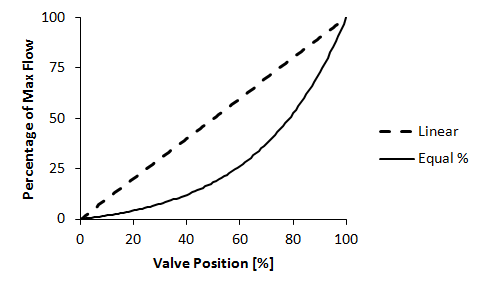
\includegraphics[width=0.55\textwidth]{Graphics/Equal-percentage.png}
	\caption{Valve characteristics}
	\label{fig:equal_percent_valve}
\end{figure}


\subsubsection{Pipe Joining Junction}
Between compressor stage 1, compressor stage 2 and the flash tank (see \cref{fig:HVAC_Diagram}) is a Pipe Joining Junction that connects the three forementioned components.

In \cref{eq:PipeJoiningJunction_ChangeOfMass}, the change of mass inside the Pipe Joining Junction can be expressed as a function of the mass flows into and out of the Pipe Joining Junction.

\begin{equation} \label{eq:PipeJoiningJunction_ChangeOfMass}
	\frac{dM}{dt} = \dot{m}_{in1} + \dot{m}_{in2} - \dot{m}_{out}
\end{equation}


where

\begin{center}
	\begin{tabular}{l p{8cm} l}
		$\dfrac{dM}{dt}$ & Change in mass inside Pipe Joining Junction		 	& [\si{kg}/\si{s}]\\
		$\dot{m}_{in1}$ & Flow into Pipe Joining Junction from Compressor $ C_1 $ 		& [\si{kg}/\si{s}]\\
		$\dot{m}_{in2}$ & Flow into Pipe Joining Junction from Flash Tank 				& [\si{kg}/\si{s}]\\
		$\dot{m_{out}}$ & Flow into Compressor $ C_2 $ from Pipe Joining Junction		& [\si{kg}/\si{s}]\\
	\end{tabular}
\end{center}

In \cref{eq:PipeJoiningJunction_Enthalpy} the specific enthalpy of the flow out of the Pipe Joining Junction is expressed as a function of the input flows and enthalpies. This equation is based on the energy balance, assuming no heat transfer to surroundings, i.e. the Pipe Joining Junction is perfectly insulated. Additionally, it is expected that $\frac{dM}{dt}$ is zero, such that the output mass flow is equal to the sum of the input flows.

\begin{equation} \label{eq:PipeJoiningJunction_Enthalpy}
	h_{out} = \frac{h_{in1} \cdot \dot{m}_{in1} + h_{in2} \cdot \dot{m}_{in2}}{ \dot{m}_{in1} + \dot{m}_{in2} }
\end{equation}

where

\begin{center}
	\begin{tabular}{l p{10cm} l}
		$h_{out}$ 			& Specific enthalpy into Compressor $ C_2 $ from Pipe Joining Junction 			& [\si{J}/\si{kg}]\\
		$h_{in1}$ 			& Specific enthalpy into Pipe Joining Junction from Compressor $ C_1 $  					& [\si{J}/\si{kg}]\\
		$h_{in2}$ 			& Specific enthalpy into Pipe Joining Junction from Flash Tank   				& [\si{J}/\si{kg}]\\
		$\dot{m}_{in1}$ 	& Flow into Pipe Joining Junction from Compressor $ C_1 $ 		& [\si{kg}/\si{s}]\\
		$\dot{m}_{in2}$ 	& Flow into Pipe Joining Junction from Flash Tank 				& [\si{kg}/\si{s}]\\
	\end{tabular}
\end{center}


%\subsubsection{Pipe Splitting Junction}

%This component is particularly simple, as the only function of it is to split the input flow in two. It is furthermore assumed that the dynamics are fast enough that the they can be modelled as algebraic equations.
%
%\begin{equation} \label{eq:PipeSplittingJunction_Enthalpy}
%	\begin{split}
%		\dot{m}_{in} &= \dot{m}_{out1} + \dot{m}_{out2} \\
%		p_{out1} &= p_{in} \\
%		p_{out2} &= p_{in} \\
%		h_{out1} &= h_{in} \\
%		h_{out1} &= h_{in} \\
%	\end{split}
%\end{equation}
%
%where
%
%\begin{center}
%	\begin{tabular}{l p{12cm} l}
%		$\dot{m}_{in}$ 		& Mass flow into Pipe Splitting Junction from Condenser (reciever?) 						& [\si{kg}/\si{s}]\\
%		$\dot{m}_{out1}$ 	& Mass flow into Economiser expansion valve from Pipe Splitting Junction 				& [\si{kg}/\si{s}]\\
%		$\dot{m}_{out2}$ 	& Mass flow into Economiser heat exchanger from Pipe Splitting Junction 					& [\si{kg}/\si{s}]\\
%		$p_{in}$ 			& Absolute pressure input Pipe Splitting Junction from Condenser (reciever?)		& [\si{Pa}]\\
%		$p_{out1}$ 			& Absolute pressure into Economiser expansion valve from Pipe Splitting Junction 	& [\si{Pa}]\\
%		$p_{out2}$ 			& Absolute pressure into Economiser heat exchanger from Pipe Splitting Junction 	& [\si{Pa}]\\
%		$h_{in}$ 			& Specific enthalpy into Pipe Splitting Junction from Condenser (reciever?)   		& [\si{J}/\si{kg}]\\
%		$h_{out1}$ 			& Specific enthalpy into Economiser expansion valve from Pipe Splitting Junction	& [\si{J}/\si{kg}]\\
%		$h_{out2}$ 			& Specific enthalpy into Economiser heat exchanger from Pipe Splitting Junction		& [\si{J}/\si{kg}]\\
%	\end{tabular}
%\end{center}
%
%
%The pressure and specific enthalpy on the output flows are equal to the input pressure and specific enthalpy. The sum of the mass flows out of the Pipe Splitting Junction is equal to the input mass flow. \\

\subsubsection{Compressor}
The compressor in the refrigeration cycle consists of two compressor stages that can be described by the same equations. The compressor type is a scroll compressor.
The compressor dynamics are assumed to be fast enough compared with the refridgeration cycle that it can be considered constant. Therefore, the equations governing the compressors are algebraic equations.
Adiabatic compression is assumed.
The two equations describing the compression governs the mass flow and the output specific enthalpy. The output specific enthalpy is found via a lookup table (HTP).

\begin{align}
	\dot{m} &= \left(\frac{V_1}{v_1} - \frac{V_C}{v_2}\right) \frac{\omega}{2} \\ \label{eq:comp_mass_flow}
	h_{out} &= \Upsilon(T_{out}, p_{out})
\end{align}

where

\begin{center}
	\begin{tabular}{l p{8cm} l}
		$\dot{m}$				& Flow through compressor stage					& [\si{kg}/\si{s}] \\
		$h_{out}$				& Compressor stage output specific enthalpy				& [\si{J}/\si{kg}] \\
		$V_1$					& Cylinder internal volume b.f. 'stroke'			& [$\si{m}^3$] \\
		$V_C$					& Cylinder clearance volume after 'stroke'		& [$\si{m}^3$] \\
		$v_1$					& Refrigerant specific volume b.f. 'stroke'		& [$\si{m}^3/\si{kg}$] \\
		$v_2$					& Refrigerant specific volume after 'stroke'		& [$\si{m}^3/\si{kg}$] \\
		$\omega$ 				& Compressor angular velocity 					& [\si{rad}/\si{s}]\\
		$\Upsilon$ 				& HTP; Lookup table of the enthalpy from temperature and pressure 			& [$\cdot]$ \\
		$T_{out}$ 				& Compressor stage output temperature 			& [\si{K}] \\
		$p_{out}$				& Compressor stage output pressure 				& [\si{Pa}]
	\end{tabular}
\end{center}

In \cref{eq:comp_mass_flow} $v_1$ is found from table lookup based on ????.

\begin{align}
	v_1 &= \Gamma(T_{in},p_{1}) \\
	v_2 &= \left(\frac{p_2}{p_1}\right)^{\frac{-1}{\gamma}} \\
	p_1 &= p_{in} - kl_1 \cdot \omega \\
	p_2 &= p_{out} + kl_2 \cdot \omega \\
	\gamma &= C_{cp}/C_{cv} \\
	T_{out} &= T_{in}\cdot \left(\frac{p_{out}}{p_{in}}\right)^{\frac{\gamma-1}{\gamma}}
\end{align}

where

\begin{center}
	\begin{tabular}{l p{8cm} l}
		$\Gamma$				& VTP; Lookup table of the specific volume from temperature and pressure		& [\si{Pa}]\\
		$p_{in}$				& Compressor stage input pressure 			& [\si{Pa}]\\
		$p_1$					& Piston input pressure									& [\si{Pa}]\\
		$p_2$					& Piston output (discharge) pressure 		& [\si{Pa}]\\
		$\gamma$				& Heat capacity ratio 								& [$ \cdot $]\\
		$ kl_1$, $kl_2$			& Valve loss constants							& [$ \cdot $]\\
		$\omega$ 				& Compressor angular velocity 				& [\si{rad}/\si{s}]\\
		$T_{in}$ 				& Compressor stage input temperature 	& [\si{K}]\\
		$C_{cp}$ 				& Specific heat capacity - constant pressure 	& [\si{J}/(\si{kg}$ \cdot $\si{K})]\\
		$C_{cv} $ 				& Specific heat capacity - constant volume 	& [\si{J}/(\si{kg}$ \cdot $\si{K})]\\
	\end{tabular}
\end{center}


%\subsubsection{Fan}
%The fans used to move air over the condenser and evaporator are driven by VFD allowing for an assumed continous range of speed settings from 0\% to 100\%. The mass flow as a function of fan speed can be modelled with a 2nd order polynomial, as shown below.
%
%The airflows over the evaporator and condenser are dynamic in themselves, as the airflow is driven by fans that have rotational inertia. Additionally, as the air is a fluid by itself, it contains some inetia too. This behaviour is modeled by:
%
%\begin{align}
%	U_* & = (U_{fan} - 2270.4)\cdot 0.0017 \\
%	\bar{\dot{V}}_{air} & = 0.7273 + 0.1202 \cdot U_*  -0.0044 \cdot U_*^2\\
%	\bar{\dot{m}}_{air} & = \bar{\dot{V}}_{air} \cdot \rho_{air}  \label{eq:Evaporator_FanAirInstantMassFlow}\\
%	%	\bar{\dot{m}}_{air} & = \frac{U_{fan}^2 \cdot 3400.5 + U_{fan}^3 \cdot -1103.5} {3600 \cdot \rho_{air}} \label{eq:Evaporator_FanAirInstantMassFlow}\\
%	\frac{\Delta \dot{m}_{air}}{\Delta t} & = \frac{\bar{\dot{m}}_{air}  - \dot{m}_{air}} {10s} \label{eq:Evaporator_FanAirRateOfChange}
%\end{align}
%
%where
%
%\begin{center}
%	\begin{tabular}{l p{8cm} l}
%		$ U_* $ 								& Intermediate variable												& [1/\si{s}]\\
%		$\bar{\dot{V}}_{air}$						& Estimated steady state volume flow of air for a given fan speed 	& [\si{m^3}/\si{s}] \\
%		$\bar{\dot{m}}_{air}$						& Estimated steady state mass flow of air for a given fan speed 	& [\si{kg}/\si{s}] \\
%		$\dot{m}_{air}$								& Actual mass flow of air					  						& [\si{kg}/\si{s}] \\
%		$U_{fan}$									& Fan speed 														& [1/\si{s}] \\
%		$\rho_{air}$								& Density of air													& [\si{kg}/\si{m^3}] \\[0.2cm]
%		$\dfrac{\Delta \dot{m}_{air}}{\Delta t} $ 	& The rate of change of	air flow 									& [\si{kg}/\si{s^2}]
%	\end{tabular}
%\end{center}
%
%\cref{eq:Evaporator_FanAirInstantMassFlow} calculates the steady state air mass flow at new speed. \cref{eq:Evaporator_FanAirRateOfChange} approximates the rate of change of the air mass flow as a first-order difference with time constant of 10 seconds. \\



\subsubsection{Condenser}

The condenser takes in the discharge pressure vapor from the second compressor stage, at point 4 in \cref{fig:HVAC_Diagram}. The high pressure also yields a high temperature,
which enables heat transfer through the condensor to ambient air. This is done mainly through condensation of the refrigerant vapor, yielding high pressure liquid at point 5 in \cref{fig:HVAC_Diagram}.
The energy balance is modelled in \cref{eq:Condenser_Enthalpy}. The mass balance is modelled in \cref{eq:Condenser_ChangeOfMass}. Finally the temperature of the metal in the condenser is modelled in
\cref{eq:Condenser_ChangeOfTemperature}, as the dominant dynamics of the condenser is greatly linked to the temperature of the metal \cite{Sorensen2013}. \cref{eq:Condenser_ChangeOfTemperature} is also
derived from the energy balance. In \cref{fig:condenser_CV} a diagram of the condenser CV can be found.

\begin{figure}[h!]
	\centering
	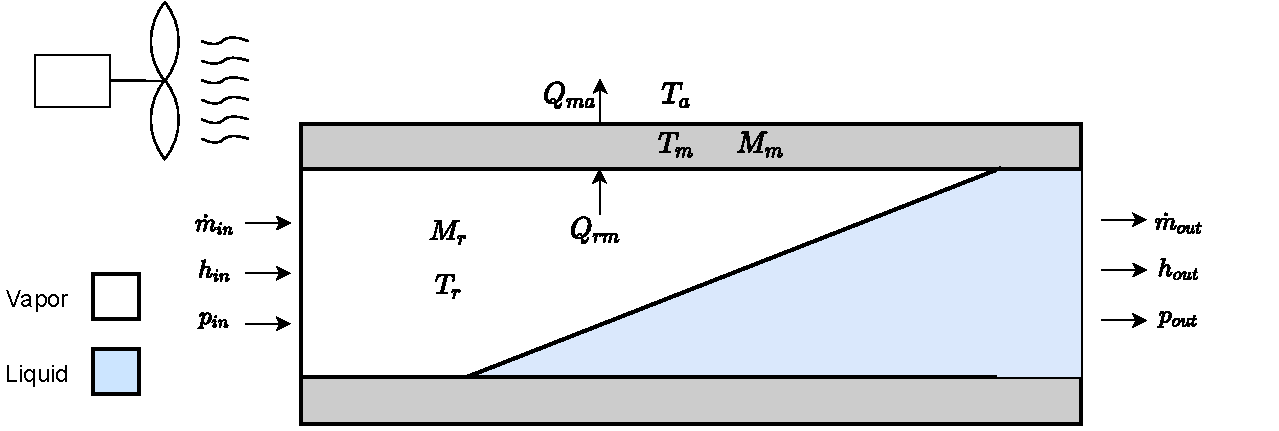
\includegraphics[width=0.8\textwidth]{Graphics/Condenser.pdf}
	\caption{Diagram of condenser control volume}
	\label{fig:condenser_CV}
\end{figure}

\begin{align}
	h_{out} 			& = h_{in} - \frac{Q_{rm}}{\dot{m}_{in}}  	\label{eq:Condenser_Enthalpy} \\
	\frac{dM_r}{dt} 	& = \dot{m}_{in} - \dot{m}_{out} 				\label{eq:Condenser_ChangeOfMass}\\
	\frac{dT_m}{dt} 	& = \frac{Q_{rm} - Q_{ma}}{M_m \cdot Cp_m}		\label{eq:Condenser_ChangeOfTemperature}
\end{align}

where

\begin{center}
	\begin{tabular}{l p{8cm} l}
		$h_{out}$				&  Condenser output specific enthalpy			& [\si{J}/\si{kg} ]\\
		$h_{in}$					&  Condenser input specific enthalpy 			& [\si{J}/\si{kg}] \\
		$Q_{rm}$					& Refrigerant to metal heat flow 			& [\si{W}] \\
		$Q_{ma}$					& Metal to air heat flow						& [\si{W}] \\
		$\dot{m_{in}}$			& Condenser input mass flow 			& [\si{kg}/\si{s}] \\
		$\dot{m_{out}}$			& Condenser output mass flow 		& [\si{kg}/\si{s}] \\
		$M_r$						& Refrigerant mass 								& [\si{kg}] \\
		$M_m$						& Metal mass												& [\si{kg}] \\
		$T_m$						& Metal temperature 							& [\si{K}]\\
		$Cp_m$					& Metal heat capacity 						& [\si{J}/\si{K}]\\
	\end{tabular}
\end{center}

The pressure drop across the condenser is assumed to be linear with respect to mass flow, yielding \cref{eq:Condenser_PressureDrop}.
The mass flow out of the condenser is modelled in \cref{eq:Condenser_MassFlow}.


\begin{align}
	p_{in} 	& =  p_{out} - \lambda \cdot \dot{m}_{in}  				\label{eq:Condenser_PressureDrop}\\
	\dot{m}_{out}		& = \dot{m}_{in} + \frac{M_r - \frac{V_i}{v}}{1s}		\label{eq:Condenser_MassFlow}
\end{align}

where

\begin{center}
	\begin{tabular}{l p{8cm} l}
		$p_{in}$				&	Condenser input pressure					& [\si{Pa}] \\
		$p_{out}$				&	Condenser output pressure					& [\si{Pa}] \\
		$\lambda$				& 	Pressure drop constant	 					& [$\cdot$] \\
		$\dot{m_{in}}$			& 	Condenser input mass flow 					& [\si{kg}/\si{s}] \\
		$\dot{m_{out}}$			& 	Condenser output mass flow 					& [\si{kg}/\si{s}] \\
		$M_{r}$					&	Condenser refridgerant mass					& [\si{kg}] \\
		$V_{i}$					&	Condenser internal volume					& [\si{m^3}] \\
		$v$						&	Condenser refridgerant specific volume		& [\si{m^3}/\si{kg}] \\
	\end{tabular}
\end{center}


And finally the convective heat flows are modelled in \cref{eq:Condenser_HeatFlow_rm}, \cref{eq:Condenser_HeatFlow_ma}. The heat flow from metal to air is assumed to be approximately proportional to the air flow, which is why the speed of the fan is multiplied to the energy flow in \cref{eq:Condenser_HeatFlow_ma}. There is an offset of 0.05 times the energy flow to account for the fact that there will exist a heat flow even though the fan is not operating.

\begin{align}
	Q_{rm}	 			& = U A_{rm} \cdot (T_r - T_m)							\label{eq:Condenser_HeatFlow_rm}\\
	Q_{ma}	 			& = U A_{ma} \cdot (T_m - T_a)\cdot (0.05 + \dfrac{U_{fan}}{1530})				\label{eq:Condenser_HeatFlow_ma}
\end{align}

where

\begin{center}
	\begin{tabular}{l p{8cm} l}
		$Q_{rm}$				&	Heat flow from refridgerant to metal					& [\si{W}] \\
		$Q_{ma}$				&	Heat flow from metal to air								& [\si{W}] \\
		$U A_{rm}$				& 	Heat transfer coefficient from refridgerant to metal 	& [\si{J}/\si{K}] \\
		$U A_{ma}$				& 	Heat transfer coefficient from metal to air				& [\si{J}/\si{K}] \\
		$T_r$					& 	Temperature of refridgerant 							& [\si{K}] \\
		$T_m$					&	Temperature of metal 									& [\si{K}] \\
		$T_a$					&	Temperature of air 										& [\si{K}] \\
		$U_{fan}$				&	Fan speed												& [1/\si{s}] \\
	\end{tabular}
\end{center}



\subsubsection{Flash tank}
The flash tank in combination with the condenser throttle valve serves to reduce the amount of high enthalpy flash gas delivered to the evaporator. The condenser throttle valve, the dynamics of which is identical to the expansion valve, lowers the pressure of the liquid from the condenser. This naturally lowers the temperature, but also generates some amount of flash gas. The flash tank then separates the liquid-vapor mixture and passes only the liquid to the expansion valve. The flash gas is returned to the second stage of the compressor, where it is reused. Thus, a lower amount of flash gas will be generated by the expansion valve, as the pressure of the liquid is already quite low.

The modeling will only evaluate the steady state behaviour of the flash tank due to the limited scope of the project. A diagram of the flash tank can be seen in \cref{fig:flash_tank_CV}

\begin{figure}[h!]
	\centering
	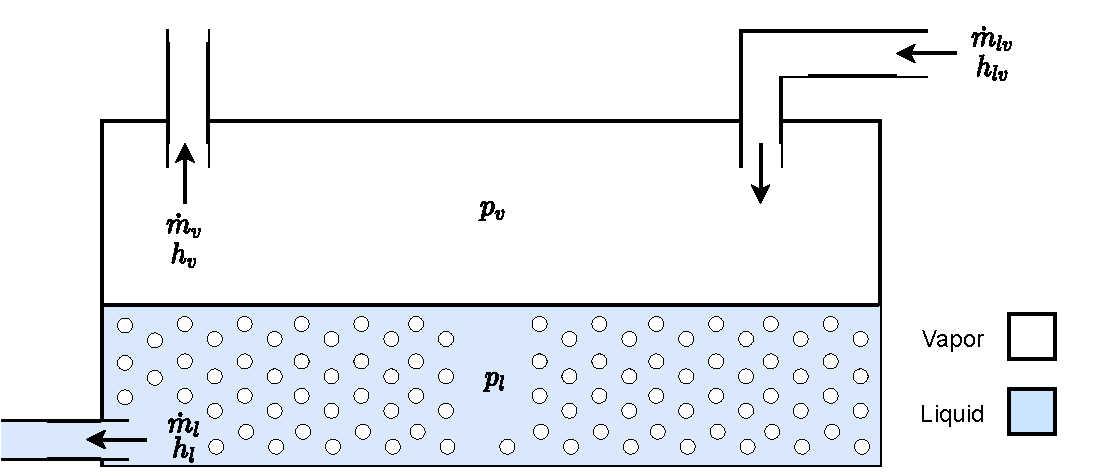
\includegraphics[width=0.65\textwidth]{Graphics/Flash_tank.pdf}
	\caption{Diagram of Flash tank control volumes}
	\label{fig:flash_tank_CV}
\end{figure}

In steady state it is first assumed that the pressure of the liquid-vapor mixture entering is the same as the separated liquid and vapor leaving the tank.
\begin{align}
	p_{lv} 	= p_{l}					&  = p_{v}
	\label{eq:Flash_tank_pressure}
\end{align}

where

\begin{center}
	\begin{tabular}{l p{8cm} l}
		$p_{lv}$				&  Liquid-vapor mixture pressure		& [\si{Pa}]\\
		$p_{l}$					&  Liquid pressure 						& [\si{Pa}] \\
		$p_{v}$					&  Vapor pressure						& [\si{Pa}]\\

	\end{tabular}
\end{center}


Secondly, it is assumed that the energy of the mixture does not change, meaning the energy flow in equals the energy flow out.
\begin{align}
	\dot{m}_{lv} \cdot  h_{lv}  - \dot{m}_{l} \cdot  h_{l} - \dot{m}_{v} \cdot  h_{v} & = 0
	\label{eq:Flash_tank_energyflow}
\end{align}

where

\begin{center}
	\begin{tabular}{l p{8cm} l}
		$\dot{m}_{lv}$			&  Liquid-vapor mixture mass flow			& [\si{kg}/\si{s}]\\
		$\dot{m}_{l}$			&  Liquid mass flow 						& [\si{kg}/\si{s}] \\
		$\dot{m}_{v}$			&  Vapor mass flow							& [\si{kg}/\si{s}]\\
		$h_{lv}$				&  Liquid-vapor mixture specific enthalpy	& [\si{J}/\si{kg}]\\
		$h_{l}$					&  Liquid specific enthalpy 				& [\si{J}/\si{kg}] \\
		$h_{v}$					&  Vapor specific enthalpy					& [\si{J}/\si{kg}]\\

	\end{tabular}
\end{center}


Lastly, it is assumed that the separated liquid and vapor leaves at boiling point and flash point respectively. This last assumption allows us to find the enthalpy of the two substances purely from investigation of the p-h diagram since the pressure is known. In practice, this is performed by a software tool as MATLAB. We express this as:

\begin{align}
	h_{l}  & = M(p)\\
	h_{v}  & = N(p)\\
\end{align}

where

\begin{center}
	\begin{tabular}{l p{8cm} l}
		$M(p)$			&  Lookup table of the enthalpy of saturated liquid	at pressure p		& [\si{J}/\si{kg}]\\
		$N(p)$			&  Lookup table of the enthalpy of saturated vapour	at pressure p		& [\si{J}/\si{kg}] \\

	\end{tabular}
\end{center}

\subsubsection{Subcooling throttle}
The subcooling throttle valve is used differently from the two other valves in the system. During normal operation it is fully open, acting as a pipe. It can be closed fully allowing for various speciel functionalities. Firstly, shutting it off allows for detecting the amount of refridgerant in the system. This is a convenient diagnostic feature which helps ensuring that the system has enough refridgerant to properly function, and enabling leakage detection. Secondly, closing the valve while fully opening the condenser throttle valve, allows the system to operate as a standard refridgeration system, with only one valve between the evaporator and condenser.


\subsubsection{Evaporator}
The superheat of the evaporator is an important and difficult state to control. It is important as the compressor can be damaged if the refrigerant contains liquid. Additionally the superheat is important from an efficiency point of view.
The superheat is the difference between the vapor saturation temperature and the actual temperature at the compressor suction inlet. It is a measure of excess energy transferred to the refrigerant.

% This clearpage might be removed. I just put it here because it was looking ugly at the time.
\clearpage

\begin{figure}[h!]
	\centering
	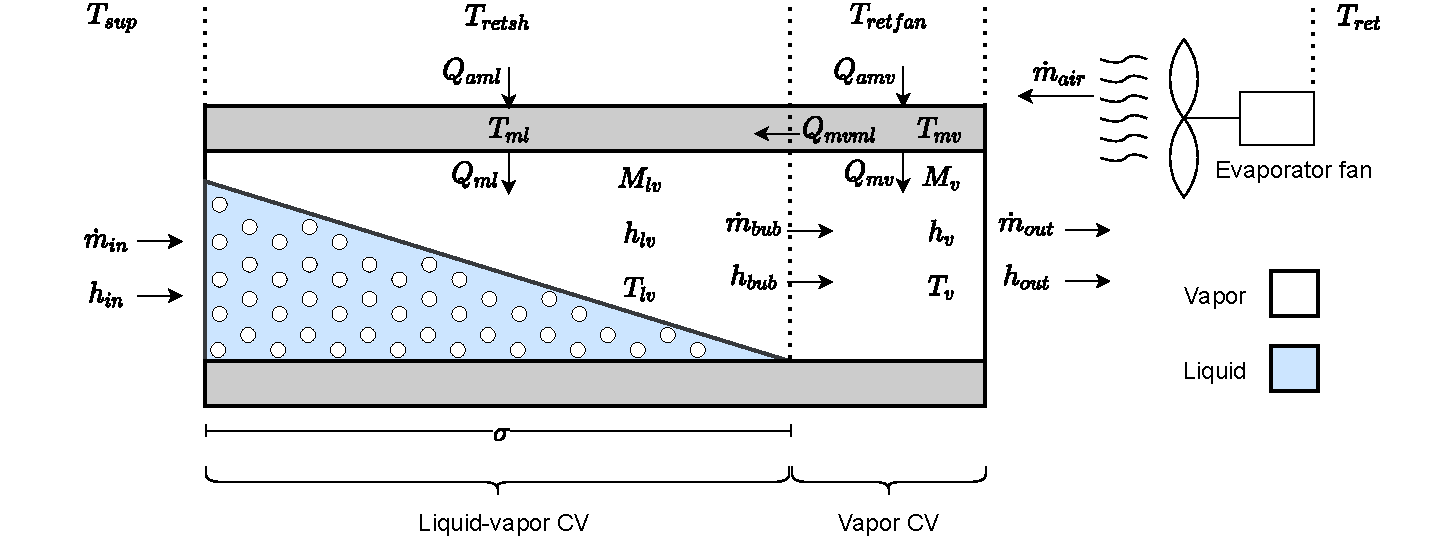
\includegraphics[width=0.8\textwidth]{Graphics/Evaporator_CV_diagram.pdf}
	\caption{Diagram of evaporator control volumes}
	\label{fig:evapo_CV}
\end{figure}

The evaporator is split into two control volumes, divided by a moving CV boundary $\sigma$ which divides liquid-vapor mixture and the superheated vapor, see \cref{fig:evapo_CV}.

Because the heat transfer coefficient between liquid and metal and vapor and metal is different, the metal is likewise split by the $\sigma$ boundary. The modeling of $\sigma$ is based on an assumption that the refrigerant has a constant average quality throughout the liquid-vapor mixture.

The calculation of the boundary location can be seen in \cref{eq:Evaporator_boundary}

\begin{equation} \label{eq:Evaporator_boundary}
	\sigma = \frac{M_l \cdot v_1}{V_i}
\end{equation}

where

\begin{center}
	\begin{tabular}{l p{8cm} l}
		$\sigma$ & Control Volume boundary                        & [$\cdot$]            \\
		$M_l$    & Mass of liquid-vapor CV                        & [\si{kg}]            \\
		$v_1$    & Refrigerant specific volume of vapor-liquid CV & [$\si{m}^3/\si{kg}$] \\
		$V_i$    & Evaporator volume                              & [$\si{m}^3$]
	\end{tabular}
\end{center}

\medskip
The temperatures of the air which is blown over the evaporator is modeled by the two equations below. The fan has some loss in the form of heat which is transferred to the air.

\begin{align}
	T_{retfan} 		& = T_{ret} + \frac{Q_{fan}}{\dot{m}_{air} \cdot Cp_{air}} 		\label{eq:T_retfan} 		\\
	T_{retsh} 		& = T_{retfan} - \frac{Q_{amv}}{\dot{m}_{air} \cdot Cp_{air}} 	\label{eq:T_retsh}
\end{align}

where

\begin{center}
	\begin{tabular}{l p{10cm} l}
		$T_{retfan}$    & Temperature of return air after passing through fan & [\si{K}]                          \\
		$T_{retsh}$     & Temperature of air over superheated vapor CV        & [\si{K}]                          \\
		$T_{ret}$       & Return temperature of air coming from trailer       & [\si{K}]                          \\
		$Q_{fan}$       & Heat added from fan to air (heatloss)               & [\si{W}]                          \\
		$Q_{amv}$       & Heat flow from air to metal surrounding vapor CV    & [\si{W}]                          \\
		$\dot{m}_{air}$ & Mass flow of air through fan                        & [\si{kg}/\si{s}]                  \\
		$Cp_{air}$      & Specific heat capacity of air                       & [\si{J}/(\si{K}$ \cdot $\si{kg})]
	\end{tabular}
\end{center}

\medskip
The heat flow from air to metal of evaporator is modeled based on the assumption that the mass flow of air is cooled down to the metal temperature as seen in \cref{eq:Q_amv} and \cref{eq:Q_aml}.

\cref{eq:Q_fan_heatloss} is the heat loss from the fan that is being added to the air flow.

\begin{align}
	U_{*_P} & = \left( \frac{U_{fan}}{3060}\cdot 100 - 55.56 \right) \cdot 0.0335 \\
	Q_{fan} & = 177.76 + 223.95 \cdot U_{*_P} + 105.85 \cdot U_{*_P}^2 + 16.74 \cdot U_{*_P}^3
	\label{eq:Q_fan_heatloss}  \\
	Q_{amv} 		& = Cp_{air} \cdot \dot{m}_{air} \cdot (T_{retfan} - T_{mv}) 	\label{eq:Q_amv} \\
	Q_{aml} 		& = Cp_{air} \cdot \dot{m}_{air} \cdot (T_{retsh} - T_{ml}) 	\label{eq:Q_aml}
\end{align}

where

\begin{center}
	\begin{tabular}{l p{10cm} l}
		$U_{*_P}$    & Scaled fan speed                                    & [1/\si{s}]                        \\
		$U_{fan}$       & Fan speed                                           & [1/\si{s}]                        \\
		$Q_{fan}$       & Heat flow from fan to air (heatloss)                & [\si{W}]                          \\
		$Q_{amv}$       & Heat flow from air to metal surrounding vapor CV    & [\si{W}]                          \\
		$Cp_{air}$      & Specific heat capacity of air                       & [\si{J}/(\si{K}$ \cdot $\si{kg})] \\
		$\dot{m}_{air}$ & Mass flow of air through fan                        & [\si{kg}/\si{s}]                  \\
		$T_{retfan}$    & Temperature of return air after passing through fan & [\si{K}]                          \\
		$T_{mv}$        & Temperature of metal on the vapor CV                & [\si{K}]
	\end{tabular}
\end{center}

The fans used to move air over the condenser and evaporator are driven by VFD allowing for an assumed continous range of speed settings from 0\% to 100\%. The mass flow as a function of fan speed can be modelled with a 2nd order polynomial, as shown below.

The airflow over the evaporator and condenser are dynamic because they are driven by fans that have rotational inertia. Additionally, as the air is a fluid itself, it contains some inertia too. This behavior is modeled by:

\begin{align}
	U_{*_{\dot{m}}} & = (U_{fan} - 2270.4)\cdot 0.0017 \\
	\bar{\dot{V}}_{air} & = 0.7273 + 0.1202 \cdot 	U_{*_{\dot{m}}}  -0.0044 \cdot 	U_{*_{\dot{m}}}^2\\
	\bar{\dot{m}}_{air} & = \bar{\dot{V}}_{air} \cdot \rho_{air}  \label{eq:Evaporator_FanAirInstantMassFlow}\\
	%	\bar{\dot{m}}_{air} & = \frac{U_{fan}^2 \cdot 3400.5 + U_{fan}^3 \cdot -1103.5} {3600 \cdot \rho_{air}} \label{eq:Evaporator_FanAirInstantMassFlow}\\
	\frac{\Delta \dot{m}_{air}}{\Delta t} & = \frac{\bar{\dot{m}}_{air}  - \dot{m}_{air}} {10s} \label{eq:Evaporator_FanAirRateOfChange}
\end{align}

where

\begin{center}
	\begin{tabular}{l p{8cm} l}
		$ 	U_{*_{\dot{m}}} $ 								& Intermediate variable												& [1/\si{s}]\\
		$\bar{\dot{V}}_{air}$						& Estimated steady state volume flow of air for a given fan speed 	& [\si{m^3}/\si{s}] \\
		$\bar{\dot{m}}_{air}$						& Estimated steady state mass flow of air for a given fan speed 	& [\si{kg}/\si{s}] \\
		$\dot{m}_{air}$								& Actual mass flow of air					  						& [\si{kg}/\si{s}] \\
		$U_{fan}$									& Fan speed 														& [1/\si{s}] \\
		$\rho_{air}$								& Density of air													& [\si{kg}/\si{m^3}] \\[0.2cm]
		$\dfrac{\Delta \dot{m}_{air}}{\Delta t} $ 	& The rate of change of	air flow 									& [\si{kg}/\si{s^2}]
	\end{tabular}
\end{center}

\cref{eq:Evaporator_FanAirInstantMassFlow} calculates the steady state air mass flow at new speed. \cref{eq:Evaporator_FanAirRateOfChange} approximates the rate of change of the air mass flow as a first-order difference with time constant of 10 seconds. \\

The temperatures of the evaporator vapor-liquid and vapor metal CVs are modeled by the two equations below respectively.

\begin{align}
	\frac{dT_{ml}}{dt} & = \frac{Q_{aml}-Q_{ml} + Q_{mvml}}{M_m \cdot Cp_m \cdot \sigma}        \\
	\frac{dT_{mv}}{dt} & = \frac{Q_{amv} - Q_{mv} - Q_{mvml}}{M_m \cdot Cp_m \cdot (1- \sigma)}
\end{align}

where

\begin{center}
	\begin{tabular}{l p{10cm} l}
		$T_{ml} $  & Metal temperature in liquid-vapor CV                                                        & [\si{K}/\si{s}]                   \\[0.3cm]
		$T_{mv} $  & Metal temperature in vapor CV                                                               & [\si{K}/\si{s}]                   \\[0.3cm]
		$Q_{aml}$  & Heat flow from air to metal surrounding liquid-vapor CV                                     & [\si{W}]                          \\
		$Q_{ml}$   & Heat flow from evaporator metal to liquid-vapor CV                                          & [\si{W}]                          \\
		$Q_{mvml}$ & Heat flow from through from metal surrounding vapor CV to metal surrounding liquid-vapor CV & [\si{W}]                          \\
		$Q_{amv}$  & Heat flow from air to metal surrounding vapor CV                                            & [\si{W}]                          \\
		$Q_{mv}$   & Heat flow from evaporator metal to vapor CV                                                 & [\si{W}]                          \\
		$M_{m} $   & Mass of metal                                                                               & [\si{kg}]                         \\
		$Cp_{m}$   & Specific heat capacity of metal                                                             & [\si{J}/(\si{K}$ \cdot $\si{kg})] \\
		$\sigma$   & Control Volume boundary                                                                     & [$\cdot$]
	\end{tabular}
\end{center}

\medskip
\cref{eq:Q_mvml}, \cref{eq:Q_ml} and \cref{eq:Q_mv} all model convection heat flows.

\begin{align}
	Q_{mvml} 		& = U A_3 \cdot (T_{mv} - T_{ml}) 								\label{eq:Q_mvml} 			\\
	Q_{ml} 			& = U A_1 \cdot (T_{ml} - T_l) \cdot \sigma						\label{eq:Q_ml} 			\\
	Q_{mv} 			& = U A_2 \cdot (T_{mv} - T_v) \cdot (1- \sigma)                \label{eq:Q_mv}
\end{align}

\begin{center}
	\begin{tabular}{l p{10cm} l}
		$Q_{aml}$       & Heat flow from air to metal surrounding liquid-vapor CV                                        & [\si{W}]                          \\
		$Q_{mvml}$      & Heat flow from through from metal surrounding vapor CV to metal surrounding liquid-vapor CV    & [\si{W}]                          \\
		$Q_{ml}$        & Heat flow from evaporator metal to liquid-vapor CV                                             & [\si{W}]                          \\
		$Q_{mv}$        & Heat flow from evaporator metal to vapor CV                                                    & [\si{W}]                          \\
		$U_{fan}$       & Fan speed                                                                                      & [1/\si{s}]                        \\
		$Cp_{air}$      & Specific heat capacity of air                                                                  & [\si{J}/(\si{K}$ \cdot $\si{kg})] \\
		$\dot{m}_{air}$ & Mass flow of air through fan                                                                   & [\si{kg}/\si{s}]                  \\
		$T_{retsh}$     & Temperature of air over superheated vapor CV                                                   & [\si{K}]                          \\
		$T_{ml}$        & Temperature of metal on the liquid-vapor CV                                                    & [\si{K}]                          \\
		$T_{mv}$        & Temperature of metal on the vapor CV                                                           & [\si{K}]                          \\
		$T_{l}$         & Saturation temperature for evaporation of the refrigerant                                      & [\si{K}]                          \\
		$T_{v}$         & Temperature of refrigerant (vapor) leaving the evaporator                                      & [\si{K}]                          \\
		$UA_1$          & Heat transfer coefficient from metal to liquid                                                 & [\si{J}/\si{K}]                   \\
		$UA_2$          & Heat transfer coefficient from metal to vapor                                                  & [\si{J}/\si{K}]                   \\
		$UA_3$          & Heat transfer coefficient from metal surrounding vapor CV to metal surrounding liquid-vapor CV & [\si{J}/\si{K}]
	\end{tabular}
\end{center}

\medskip
Output pressure, specific enthalpies and mass balances are given by equations \cref{eq:evap_pout} $\rightarrow$ \cref{eq:evap_dMvdt}. \cref{eq:evap_Tsup} describes the temperature of the air leaving the evaporator and \cref{eq:evap_mdot_lv} describes the flow from the liquid-vapor CV to the vapor CV. The dew point specific enthalpy is the point at the evaporator pressure where liquid turns to vapor.

\begin{align}
	p_{out}         & = \Pi \left( h_v, \frac{V_i-V_l}{M_v} \right)		\label{eq:evap_pout}                       \\
	h_{lv}             & = h_{in} + \frac{Q_{ml}}{\dot{m}_{in}}                                                       \\
	h_v             & = h_{dew} + \frac{Q_{mv}}{\dot{m}_{lv}}                                                       \\
	\frac{dM_l}{dt} & = \dot{m}_{in} - \dot{m}_{lv}                                                                \\
	\frac{dM_v}{dt} & = \dot{m}_{lv} - \dot{m}_{out}                   \label{eq:evap_dMvdt}                       \\
	T_{sup}         & = T_{retfan} +  \frac{Q_{aml} + Q_{amv}}{Cp_{air} \cdot \dot{m}_{air}} \label{eq:evap_Tsup} \\
	\dot{m}_{lv}    & = \frac{Q_{ml}}{h_{dew} - h_{in}} \label{eq:evap_mdot_lv}
\end{align}



where\\


\begin{center}
	\begin{tabular}{l p{10cm} l}
		$ p_{out} 	$     & Pressure in evaporator                                                  & [\si{Pa}]                         \\
		$\Pi(h,\rho) $   & Table lookup of pressure, where inputs are specific enthalpy and density & [\si{Pa}]                         \\
		$h_{v} $         & Specific enthalpy of vapor CV                                            & [\si{J}/\si{kg}]                  \\
		$h_{lv} $         & Specific enthalpy of liquid-vapor CV                                     & [\si{J}/\si{kg}]                  \\
		$h_{in} $        & Specific enthalpy of input liquid refrigerant                            & [\si{J}/\si{kg}]                  \\
		%$h_{lv} $        & Specific enthalpy of refrigerant moving from liquid-vapor CV to vapor CV & [\si{J}/\si{kg}]                  \\
		$h_{dew}$        & Specific enthalpy of dew point                                           & [\si{J}/\si{kg}]                  \\
		$V_{i} $         & Total volume of evaporator                                               & [\si{m^3}]                        \\
		$V_{l} $         & Volume of liquid refrigerant                                             & [\si{m^3}]                        \\
		$M_{v}$          & Mass in	in vapor CV                                                     & [\si{kg}/\si{s}]                  \\
		$M_{l}$          & Mass in	in liquid-vapor CV                                              & [\si{kg}/\si{s}]                  \\
		$Q_{ml}$         & Heat flow from evaporator metal to liquid-vapor CV                       & [\si{W}]                          \\
		$Q_{mv}$         & Heat flow from evaporator metal to vapor CV                              & [\si{W}]                          \\
		$Q_{aml}$        & Heat flow from air to metal surrounding liquid-vapor CV                  & [\si{W}]                          \\
		$Q_{amv}$        & Heat flow from air to metal surrounding vapor CV                         & [\si{W}]                          \\
		$M_{m}$          & Mass of metal                                                            & [\si{kg}]                         \\
		$M_{v}$          & Mass of vapor                                                            & [\si{kg}]                         \\
		$Cp_{air}$       & Specific heat capacity of air                                            & [\si{J}/(\si{K}$ \cdot $\si{kg})] \\
		$\dot{m}_{in} $  & Mass flow of input refrigerant                                           & [\si{kg}/\si{s}]                  \\
		$\dot{m}_{lv} $  & Mass flow of refrigerant from liquid-vapor CV to vapor CV                & [\si{kg}/\si{s}]                  \\
		$\dot{m}_{out} $ & Mass flow of output refrigerant                                          & [\si{kg}/\si{s}]                  \\
		$\dot{m}_{air}$  & Actual mass flow of air                                                  & [\si{kg}/\si{s}]                  \\
		$T_{sup} $       & Temperature of air flowing into trailer box                              & [\si{K}]                          \\
		$T_{retfan}$     & Temperature of return air after passing through fan                      & [\si{K}]
	\end{tabular}
\end{center}


\subsubsection{Box}
The trailer box contains by far the greatest thermodynamic capacities due to the large mass of the cargo. The cargo temperature is strongly coupled to the surrounding air temperature due to its large surface area. The temperatures of the two main thermal capacities are modeled and their state space equations are given as below:

\begin{align}
	\frac{dT_{air}}{dt} & = \frac{Q_{ca} + Q_{ba} + Q_{fan} -Q_{cool}}{M_{air} \cdot Cp_{air}} \\
	\frac{dT_{box}}{dt} & = \frac{Q_{amb} - Q_{ba}}{M_{box} \cdot Cp_{box}} \\
	\frac{dT_{cargo}}{dt} & = \frac{-Q_{ca}}{M_{cargo} \cdot Cp_{cargo}}
\end{align}

where
\begin{center}
	\begin{tabular}{l p{8cm} l}
		$Q_{ca}$     & Cargo to air heat flow       & [\si{W}]                \\
		$Q_{ba}$     & Box to air heat flow         & [\si{W}]                \\
		$Q_{fan}$    & Fan to air heat flow         & [\si{W}]                \\
		$Q_{cool}$   & Air to evaporator heat flow  & [\si{W}]                \\
		$Q_{amb}$    & Ambient to box heat flow     & [\si{W}]                \\
		$T_{air}$    & Air temperature              & [\si{K}]                \\
		$T_{box}$    & Box temperature              & [\si{K}]                \\
		$T_{cargo}$  & Cargo temperature            & [\si{K}]                \\
		$M_{air}$    & Air mass                     & [\si{kg}]               \\
		$M_{box}$    & Trailer box aluminum mass    & [\si{kg}]               \\
		$M_{cargo}$  & Cargo mass                   & [\si{kg}]               \\
		$Cp_{air}$   & Air specific heat capacity   & [\si{J}/\si{kg} \si{K}] \\
		$Cp_{cargo}$ & Cargo specific heat capacity & [\si{J}/\si{kg} \si{K}] \\
		$Cp_{box}$   & Cargo specific heat capacity & [\si{J}/\si{kg} \si{K}]
	\end{tabular}
\end{center}

%where
%\begin{center}
%	\begin{tabular}{l p{8cm} l}
	%		$Q_{ca}$			& Cargo to air heat flow					& [\si{W}] \\
	%		$Q_{aa}$			& Ambient (walls and roof) to air heat flow		& [\si{W}] \\
	%		$Q_{fa}$			& Floor to air heat flow 						& [\si{W}] \\
	%		$Q_{af}$			& Ambient (floor) to floor heat flow 	& [\si{W}] \\
	%		$Q_{fan}$			& Fan to air heat flow 						& [\si{W}] \\
	%		$Q_{cool}$			& Air to evaporator heat flow  			& [\si{W}] \\
	%		$T_{air}$			& Air temperature 								& [\si{K}] \\
	%		$T_{floor}$			& Floor temperature						& [\si{K}] \\
	%		$T_{cargo}$		& Cargo temperature							& [\si{K}] \\
	%		$M_{air}$			& Air mass										& [\si{kg}] \\
	%		$M_{floor}$			& Floor mass								& [\si{kg}] \\
	%		$M_{cargo}$		& Cargo mass								& [\si{kg}] \\
	%		$Cp_{air}$			& Air heat capacity							& [\si{J}/\si{kg} \si{K}] \\
	%		$Cp_{floor}$	& Floor heat capacity						& [\si{J}/\si{kg} \si{K}] \\
	%		$Cp_{cargo}$	& Cargo heat capacity					& [\si{J}/\si{kg} \si{K}]
	%	\end{tabular}
%\end{center}

The heat flows are modeled as seen in \cref{eq:box_Qcool} $\rightarrow$ \cref{eq:box_Qfan}. $ U_* $ in \cref{eq:box_Uscaled} is simply an intermediate scaled fan speed used in modeling the fan heat loss $ Q_{fan} $.

\begin{align}
	Q_{cool}   & = Cp_{air} \cdot \dot{m_{air}} \cdot (T_{ret} - T_{sup})	\label{eq:box_Qcool}                                 \\
	Q_{amb}    & = (T_{ambi} - T_{box}) \cdot U A_{amb}						\label{eq:box_Qab}                                                \\
	Q_{ba}     & = (T_{box} - T_{air}) \cdot U A_{ba}						\label{eq:box_Qba}                                                  \\
	Q_{ca}     & = (T_{cargo} - T_{air}) \cdot U A_{cargo}                                                                     \\
	Q_{fan}    & = 177.76 + 223.95 \cdot U_* + 105.85 \cdot U_*^2 + 16.74 \cdot U_*^3 \label{eq:box_Qfan} \\
	U_* & = \left( \frac{U_{fan}}{3060}\cdot 100 - 55.56 \right) \cdot 0.0335 \label{eq:box_Uscaled}
\end{align}

where
\begin{center}
	\begin{tabular}{l p{8cm} l}
		$\dot{m}_{air}$ & Air mass flow                                & [\si{kg}/{\si{s}}] \\
		$T_{ret}$       & Return air temperature                       & [\si{K}]           \\
		$T_{sup}$       & Supply air temperature                       & [\si{K}]           \\
		$T_{ambi}$      & Ambient air temperature                      & [\si{K}]           \\
		$T_{box}$       & Box aluminum temperature                     & [\si{K}]           \\
		$U A_{amb}$     & Ambient air to box heat transfer coefficient & [\si{W}/\si{K}]    \\
		$U A_{ba}$      & Box to air heat transfer coefficient         & [\si{W}/\si{K}]    \\
		$U A_{cargo}$   & Cargo to air heat transfer coefficient       & [\si{W}/\si{K}]    \\
		$U_{fan}$       & Fan speed                                    & [$\cdot$]          \\
		$U_*$    & Scaled fan speed                             & [$\cdot$]
	\end{tabular}
\end{center}

$Q_{cool}$ is the cooling provided by the evaporator. It is calculated based on the difference between the temperature of the air returning from the box ($T_{ret}$) and the temperature of the air supplied to the box $T_{sup}$ as seen in \cref{eq:box_Qcool}

\clearpage
\newpage
\subsection{Collection of components}

\begin{figure}[h!]
	\centering
	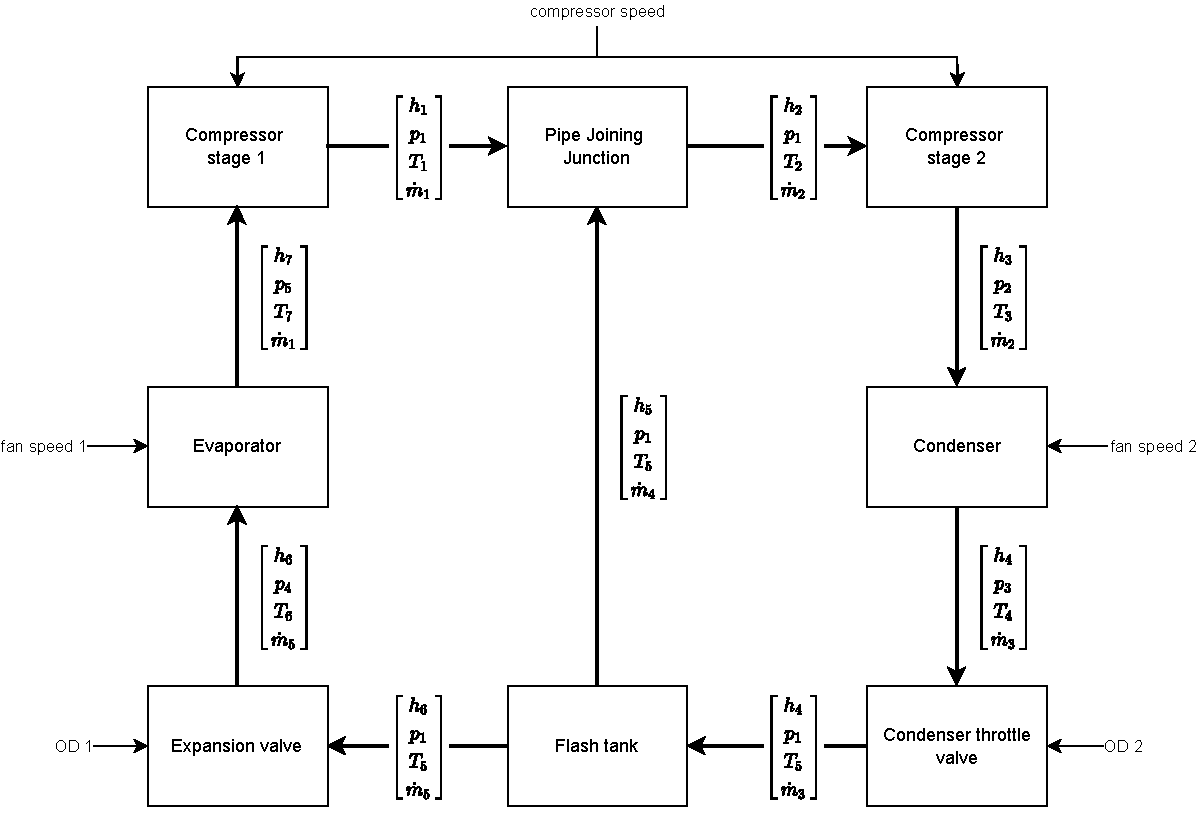
\includegraphics[width=1\textwidth]{Graphics/Block_Diagram.pdf}
	\caption{Initial Block Diagram with states}
	\label{fig:Block_diagram}
\end{figure}


\begin{equation} \label{eq:f_noSub} \renewcommand{\arraystretch}{2.4}
	f(x,u) =  \dfrac{d}{dt} \begin{bmatrix}
		M_{pjj}		\\					%pjj
		M_{condenser} 	\\				%condenser
		T_m 			\\				%condenser
		\dot{m}_{air}	\\				%evaporator
		T_{ml}			\\				%evaporator
		T_{mv}			\\				%evaporator
		M_l				\\				%evaporator
		M_v				\\				%evaporator
	\end{bmatrix}
	=
	\begin{bmatrix}
		\dot{m}_1 + \dot{m}_4 - \dot{m}_2 \\										%pjj
		\dot{m}_{2} - \dot{m}_{3}	\\												%condenser
		\dfrac{Q_{rm} - Q_{ma}}{M_m \cdot Cp_m} \\									%condenser
		\dfrac{\bar{\dot{m}}_{air}  - \dot{m}_{air}} {10s}		\\					%evaporator
		\dfrac{Q_{aml}-Q_{ml} + Q_{mvml}}{M_m \cdot Cp_m \cdot \sigma}        \\	%evaporator
		\dfrac{Q_{amv} - Q_{mv} - Q_{mvml}}{M_m \cdot Cp_m \cdot (1- \sigma)}	\\	%evaporator
		\dot{m}_{5} - \dot{m}_{lv}		\\											%evaporator
		\dot{m}_{lv} - \dot{m}_{1}	\\												%evaporator
	\end{bmatrix}
\end{equation}






\begin{equation} \label{eq:f_Sub} \renewcommand{\arraystretch}{3.4}
	f(x,u) =   \dfrac{d}{dt} \begin{bmatrix}
		M_{_{PJJ}}		\\				%pjj
		M_{Con} 		\\				%condenser
		T_m 			\\				%condenser
		\dot{m}_{air}	\\				%evaporator
		T_{ml}			\\				%evaporator
		T_{mv}			\\				%evaporator
		M_l				\\				%evaporator
		M_v				\\				%evaporator
	\end{bmatrix}
	=
	\begin{bmatrix}
		\left(\dfrac{V_1}{v_{1_{COM1}}} - \dfrac{V_C}{v_{2_{COM1}}}\right) \dfrac{\omega}{2} + \dfrac{\dot{m}_{3} \cdot h_4 - \dot{m}_{5} \cdot h_6}{h_5} - \left(\dfrac{V_1}{v_{1_{COM2}}} - \dfrac{V_C}{v_{2_{COM2}}}\right) \dfrac{\omega}{2} \\										%pjj
		\left(\dfrac{V_1}{v_{1_{COM2}}} - \dfrac{V_C}{v_{2_{COM2}}}\right) \dfrac{\omega}{2} - f_p(\Theta_1) \cdot K  \sqrt{\dfrac{1}{v_{_{CTV_{in}}}} (p_{3} - p_{1})}	\\												%condenser
		\dfrac{U A_{rm} \cdot (T_r - T_m) - U A_{ma} \cdot (T_m - T_a)\cdot \left(0.05 + \dfrac{U_{fan_1}}{1530}\right)}{M_m \cdot Cp_m} \\									%condenser
		\dfrac{\left( 0.7273 + 0.1202 \cdot U_{*_{\dot{m}}}  -0.0044 \cdot	U_{*_{\dot{m}}}^2 \right) \cdot \rho_{air}  - \dot{m}_{air}} {10s}		\\					%evaporator
		\dfrac{Cp_{air} \cdot \dot{m}_{air} \cdot (T_{retsh} - T_{ml})-U A_1 \cdot (T_{ml} - T_l) \cdot \sigma + U A_3 \cdot (T_{mv} - T_{ml})}{M_m \cdot Cp_m \cdot \sigma}        \\	%evaporator
		\dfrac{Cp_{air} \cdot \dot{m}_{air} \cdot (T_{retfan} - T_{mv}) - U A_2 \cdot (T_{mv} - T_v) \cdot (1- \sigma) - U A_3 \cdot (T_{mv} - T_{ml})}{M_m \cdot Cp_m \cdot (1- \sigma)}	\\	%evaporator
		f_p(\Theta_2) \cdot K  \sqrt{\dfrac{1}{v_{_{EV_{in}}}} (p_{1} - p_{4})} - \dfrac{U A_1 \cdot (T_{ml} - T_l) \cdot \sigma}{h_{dew} - h_{6}}		\\											%evaporator
		\dfrac{U A_1 \cdot (T_{ml} - T_l) \cdot \sigma}{h_{dew} - h_{6}} - \left(\dfrac{V_1}{v_{1_{COM1}}} - \dfrac{V_C}{v_{2_{COM1}}}\right) \dfrac{\omega}{2}	\\												%evaporator
	\end{bmatrix}
\end{equation}





\begin{equation} \label{eq:Gpjj}\renewcommand{\arraystretch}{2.5}
	g_{_{PJJ}}(x,u) =  \begin{bmatrix}
		h_{2}				\\ %pjj
		\dot{m}_{2}			\\ %pjj
	\end{bmatrix}
	-
	\begin{bmatrix}
		\dfrac{h_{1} \cdot \dot{m}_{1} + h_{5} \cdot \dot{m}_{4}}{ \dot{m}_{2} } \\ 	%pjj
		\dot{m}_{1} + \dot{m}_{4} \\													%pjj
	\end{bmatrix}
	=\textbf{0}
\end{equation}


\begin{equation} \label{eq:Gcs2}\renewcommand{\arraystretch}{2.5}
	g_{_{COM2}}(x,u) =  \begin{bmatrix}
		\dot{m}_2  		 	\\ %COM2
		h_{3}				\\ %COM2
		v_{1_{COM2}}			\\ %COM2
		v_{2_{COM2}}			\\ %COM2
		p_{i1_{COM2}}		\\ %COM2
		p_{i2_{COM2}}		\\ %COM2
		\gamma				\\ %COM2
		T_{3}				\\ %COM2
	\end{bmatrix}
	-
	\begin{bmatrix}
		\left(\dfrac{V_1}{v_{1_{COM2}}} - \dfrac{V_C}{v_{2_{COM2}}}\right) \dfrac{\omega}{2} \\			%COM2
		\Upsilon(T_{3}, p_{2})		\\													%COM2
		\Gamma(T_{2},p_{i1_{COM2}}) \\													%COM2
		\left(\dfrac{p_{i2_{COM2}}}{p_{i1_{COM2}}}\right)^{\frac{-1}{\gamma}} \\		%COM2
		p_{1} - kl_1 \cdot \omega \\													%COM2
		p_{2} + kl_2 \cdot \omega \\													%COM2
		\dfrac{C_{cp}}{C_{cv}} \\														%COM2
		T_{2}\cdot \left(\dfrac{p_{2}}{p_{1}}\right)^{\frac{\gamma-1}{\gamma}}	\\		%COM2
	\end{bmatrix}
	=\textbf{0}
\end{equation}


\begin{equation} \label{eq:Gcondenser}\renewcommand{\arraystretch}{2.5}
	g_{_{Con}}(x,u) =  \begin{bmatrix}
		h_{4}				\\ %condenser
		p_{2}				\\ %condenser
		\dot{m}_{3}			\\ %condenser
		Q_{rm}				\\
		Q_{ma}				\\
	\end{bmatrix}
	-
	\begin{bmatrix}
		h_{3} - \dfrac{Q_{rm}}{\dot{m}_{2}}	\\											%condenser
		p_{3} - \lambda \cdot \dot{m}_{2}			\\									%condenser
		\dot{m}_{2} + \dfrac{M_{con} - \frac{V_i}{v_{Con}}}{1s}	\\						%condenser
		U A_{rm} \cdot (T_r - T_m) \\
		U A_{ma} \cdot (T_m - T_a)\cdot \left(0.05 + \dfrac{U_{fan_1}}{1530}\right) \\
	\end{bmatrix}
	=\textbf{0}
\end{equation}




\begin{equation} \label{eq:Gvalves}\renewcommand{\arraystretch}{2.5}
	g_{_{Val}}(x,u) =  \begin{bmatrix}
		\dot{m}_{3}			\\ %condenser valve

		\dot{m}_{5}			\\ %expansion valve
	\end{bmatrix}
	-
	\begin{bmatrix}
		f_p(\Theta_1) \cdot K  \sqrt{\dfrac{1}{v_{_{CTV_{in}}}} (p_{3} - p_{1})}\\		%condenser valve
		f_p(\Theta_2) \cdot K  \sqrt{\dfrac{1}{v_{_{EV_{in}}}} (p_{1} - p_{4})}\\			%expansion valve
	\end{bmatrix}
	=\textbf{0}
\end{equation}

\begin{equation} \label{eq:Gflashtank}\renewcommand{\arraystretch}{2.5}
	g_{_{FT}}(x,u) =  \begin{bmatrix}
		\dot{m}_{4}			\\
		\dot{m}_{5}				\\
		h_{5}  \\
		h_{6} \\
	\end{bmatrix}
	-
	\begin{bmatrix}
		\dfrac{\dot{m}_{3} \cdot h_4 - \dot{m}_{5} \cdot h_6}{h_5}					\\
		\dot{m}_{3} - \dot{m}_{4}					\\
		N(p_1)\\
		M(p_1)\\
	\end{bmatrix}
	=\textbf{0}
\end{equation}



\begin{equation} \label{eq:Gevaporator}\renewcommand{\arraystretch}{2.5}
	g_{_{Eva}}(x,u) =  \begin{bmatrix}
		\sigma		\\
		T_{retfan}	\\
		T_{retsh}	\\
		U_{*_P}	\\
		Q_{fan_2}		\\
		Q_{amv}		\\
		Q_{aml}		\\
		U_{*_{\dot{m}}}	\\
		\bar{\dot{V}}_{air}		\\
		\bar{\dot{m}}_{air}		\\
		Q_{mvml}	\\
		Q_{ml}		\\
		Q_{mv}		\\
		p_{5}		\\
		h_{lv}			\\
		h_v 		\\
		T_{sup}		\\
		\dot{m}_{lv}\\
	\end{bmatrix}
	-
	\begin{bmatrix}
		\dfrac{M_l \cdot v_{_{Eva}}}{V_i}							\\
		T_{ret} + \dfrac{Q_{fan_2}}{\dot{m}_{air} \cdot Cp_{air}}			\\
		T_{retfan} - \dfrac{Q_{amv}}{\dot{m}_{air} \cdot Cp_{air}}		\\
		\left( \dfrac{U_{fan_2}}{3060}\cdot 100 - 55.56 \right) \cdot 0.0335 \\
		177.76 + 223.95 \cdot U_{*_P} + 105.85 \cdot U_{*_P}^2 + 16.74 \cdot U_{*_P}^3 \\
		Cp_{air} \cdot \dot{m}_{air} \cdot (T_{retfan} - T_{mv}) 	 \\
		Cp_{air} \cdot \dot{m}_{air} \cdot (T_{retsh} - T_{ml}) \\
		(U_{fan_2} - 2270.4)\cdot 0.0017 \\
		0.7273 + 0.1202 \cdot 	U_{*_{\dot{m}}}  -0.0044 \cdot	U_{*_{\dot{m}}}^2\\
		\bar{\dot{V}}_{air} \cdot \rho_{air}	\\
		U A_3 \cdot (T_{mv} - T_{ml})	\\
		U A_1 \cdot (T_{ml} - T_l) \cdot \sigma	\\
		U A_2 \cdot (T_{mv} - T_v) \cdot (1- \sigma)	\\
		\Pi \left( h_v, \dfrac{V_i-V_l}{M_v} \right)		\\
		h_{6} + \dfrac{Q_{ml}}{\dot{m}_{5}}			\\
		h_{dew} + \dfrac{Q_{mv}}{\dot{m}_{lv}}   		\\
		T_{retfan} +  \dfrac{Q_{aml} + Q_{amv}}{Cp_{air} \cdot \dot{m}_{air}} \\
		\dfrac{Q_{ml}}{h_{dew} - h_{6}}		\\
	\end{bmatrix}
	=\textbf{0}
\end{equation}



\begin{equation} \label{eq:Gcs1}\renewcommand{\arraystretch}{2.5}
	g_{_{COM1}}(x,u) =  \begin{bmatrix}
		\dot{m}_1  		 	\\ %COM1
		h_{1}				\\ %COM1
		v_{1_{COM1}}			\\ %COM1
		v_{2_{COM1}}			\\ %COM1
		p_{i1_{COM1}}		\\ %COM1
		p_{i2_{COM1}}		\\ %COM1
		\gamma				\\ %COM1
		T_{1}				\\ %COM1
	\end{bmatrix}
	-
	\begin{bmatrix}
		\left(\dfrac{V_1}{v_{1_{COM1}}} - \dfrac{V_C}{v_{2_{COM1}}}\right) \dfrac{\omega}{2} \\			%COM1
		\Upsilon(T_{1}, p_{1})		\\													%COM1
		\Gamma(T_{7},p_{i1_{COM1}}) \\													%COM1
		\left(\dfrac{p_{i2_{COM1}}}{p_{i1_{COM1}}}\right)^{\frac{-1}{\gamma}} \\		%COM1
		p_{5} - kl_1 \cdot \omega \\													%COM1
		p_{1} + kl_2 \cdot \omega \\													%COM1
		\dfrac{C_{cp}}{C_{cv}} \\												%COM1
		T_{7}\cdot \left(\dfrac{p_{1}}{p_{5}}\right)^{\frac{\gamma-1}{\gamma}}	\\		%COM1
	\end{bmatrix}
	=\textbf{0}
\end{equation}


\begin{equation} \label{eq:Gtotal}\renewcommand{\arraystretch}{2.5}
	g(x,u) =  \begin{bmatrix}
		g_{_{PJJ}}(x,u)  		 	\\ %COM1
		g_{_{COM2}}(x,u)				\\ %COM1
		g_{_{Con}}(x,u)			\\ %COM1
		g_{_{Val}}(x,u)			\\ %COM1
		g_{_{FT}}(x,u)		\\ %COM1
		g_{_{Eva}}(x,u)		\\ %COM1
		g_{_{COM1}}(x,u)			\\
	\end{bmatrix}
	= \textbf{0}
\end{equation}




\newpage
\subsubsection{Linearisation}